% Created: Enze Chen, June 2025
%
% Chapter 10 of the MSE 142 coursereader. This chapter introduces the notion of indistinguishability and exchange (e.g., Pauli exclusion principle), leading to a discussion of topology and group theory.

% Uncomment the following three lines and last line to individually compile this chapter
\documentclass[12pt, english]{book}
\usepackage{142crstyle}
\begin{document}

\chapter[Topology]{Work in Progress:\\Topology and Indistinguishability} \label{ch:topo}
%{ \doublespacing 
As an advanced topic, we'll discuss the distinguishability (or lack thereof) of quantum particles and their topology.
While they sound abstract, these concepts are important for...
We'll just sketch the main ideas here, and encourage you to consult other resources for a more thorough treatment.


%%%%%%%%%%%%%%%%%%%%%%%%%%%%%%%%%%%%%%%%%%%%%%%%%%%%%%%%%%%%%%%%%%%%%%%%%%%%%%%%

\section{Before you begin}

This chapter builds on the following concepts, some of which we've already discussed in class, others you will likely have encountered elsewhere.
We include links to resources that may aid your review, as mastery of these concepts will allow you to get the most out of this chapter.

\begin{itemize}
	\item foo 
	\item bar 
	\item Prerequisite self-check quiz 
\end{itemize}


%%%%%%%%%%%%%%%%%%%%%%%%%%%%%%%%%%%%%%%%%%%%%%%%%%%%%%%%%%%%%%%%%%%%%%%%%%%%%%%%

\section{Fermions and bosons}

To start off, imagine we have a wave function for a two-particle system, $\Psi(x_1, x_2)$.
If the two particles are indistinguishable, then their probability densities, given by $\abs{\Psi}^2$, should be \textbf{invariant under exchange}.
That is, if the two particles swapped places, we wouldn't be able to tell the difference.
Mathematically, we would write

\begin{equation}
	\abs{\Psi(x_1, x_2)}^2 = \abs{\Psi(x_2, x_1)}^2  \label{eq:swapped}
\end{equation}

The consequence of Equation~\ref{eq:swapped} is that the two wave functions are only off by a multiplicative constant,

\begin{equation}
	\Psi(x_1, x_2) = A \Psi(x_2, x_1)
	\label{eq:swapped_A}
\end{equation}

where $A = e^{i \alpha}$ for some phase $\alpha$.
Now consider further a situation of \emph{double exchange}, where the two particles return to their initial positions. 
If this is true, then we should obtain the original wave function.
Now using Equation~\ref{eq:swapped_A}, we get
\begin{align*}
	\Psi(x_1, x_2) &= A \Psi(x_2, x_1) \\
	\Psi(x_1, x_2) &= A^2  \Psi(x_1, x_2) \\
	A^2 &= 1 \\
	A = e^{i \alpha} &= \pm 1   \numberthis \label{eq:swapped_pm}
\end{align*}

Equation~\ref{eq:swapped_pm} gives us two classes of particles:

\begin{tcolorbox}[title = Fermions]
	$e^{i \alpha} = -1$ describes \textbf{fermions}, which are \emph{antisymmetric} under exchange, $\Psi(x_1, x_2) = - \Psi(x_2, x_1)$.
	Electrons are common examples of fermions.
\end{tcolorbox}

\begin{tcolorbox}[title = Bosons]
	$e^{i \alpha} = 1$ describes \textbf{bosons}, which are \emph{symmetric} under exchange, $\Psi(x_1, x_2) = \Psi(x_2, x_1)$.
	Photons and phonons are common examples of bosons.
\end{tcolorbox}

Fermions have a particularly interesting probability with respect to their indistinguishability.
Imagine the two particles are in the same single-particle state, such that $x_1 = x_2$.
Then we have 

\begin{equation}
	\Psi(x_1, x_1) = -\Psi(x_1, x_1) \implies \Psi(x_1, x_1) = 0   \label{eq:pauli}
\end{equation}

If the wave function is 0 everywhere, then the probability of this configuration is also 0.
Equation~\ref{eq:pauli} leads to the celebrated Pauli exclusion principle.

\begin{tcolorbox}[title = Pauli exclusion principle]
	It is \textbf{impossible} for two fermions to occupy the same quantum state.
\end{tcolorbox}

For fermions, this sign change upon exchange underlies the origins of semiconductors, metals, atomic structure, neutron stars, the periodic table, etc.
Spin statistics connection: Fermions have half-integer spin (e.g., electrons are spin $\frac{1}{2}$) while bosons have integer spin (e.g., photons).

\begin{figure}[!ht]
	\centering 
	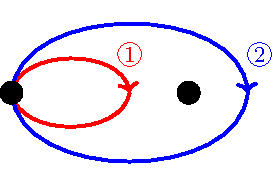
\includegraphics[width=0.35\linewidth]{exchange-paths.pdf}
	\caption{Topological viewpoint of exchange, where Path 1 does not carry out exchange and can be contracted to the pull path, but Path 2 carries out double exchange.}
	\label{fig:exchange}
\end{figure}

Let us now provide a topological picture of exchange, which we'll describe in more detail in the following section.
Consider a system of two indistinguishable electrons arranged as in \autoref{fig:exchange}.
In the figure are also two paths that represent processes that operate on the position of the left particle.
Along Path 1, there is no exchange, as in one sense the particle has not changed its relative position, but more importantly, this path can be contracted (deformed) into the single particle (a null operation, in some sense).

Path 2, on the other hand, corresponds to double exchange, as halfway through, the particles have switched places, and by the end they have switched back.
Moreover, in 3D, it is possible to physically deform path 2 to match path 1 (lift it out of the plane of the paper), so double exchange is equivalent to no exchange.
They have the same topological properties (such paths are called \emph{homotopic}), which admits $e^{2 i \alpha} = 1$, as seen earlier in \autoref{eq:swapped_pm}.

But in 2D, these paths cannot be deformed continuously to match each other, and the paths are knotted!
This means in 2D, double exchange is \emph{not} equivalent to no exchange and that $e^{2 i \alpha}$ does not necessarily equal 1.
This describes a class of particles called \textbf{anyons}, which are the basis for topological quantum computing.\footnote{See the article by V. Lahtinen and J. Pachos, \href{https://arxiv.org/abs/1705.04103}{\emph{SciPost Physics}} 3, 2017, for a lengthier introduction to this topic.}


%%%%%%%%%%%%%%%%%%%%%%%%%%%%%%%%%%%%%%%%%%%%%%%%%%%%%%%%%%%%%%%%%%%%%%%%%%%%%%%%

\section{Topology}

Topology is the study of the \emph{global} properties of geometric objects that don't depend on local features, or are \emph{preserved} under small local deformations.
A canonical example is the topological equivalency of a donut and a mug.
Although the two objects look very different, they are topologically very similar (equivalent, in fact) because both feature a single hole---the donut through the center and the mug through the handle.\footnote{You can read more about topology in \href{https://phys.org/news/2016-10-coffee-donut-topology.html}{this Phys.org article} discussing the \href{https://www.nobelprize.org/prizes/physics/2016/summary/}{2016 Nobel Prize in Physics} on topological phase transitions.}
As a result, it is possible to continuously deform one shape into the other, as seen \href{https://tex.stackexchange.com/questions/210255/torus-to-coffee-mug-homotopy}{in this animation}.
Contrast these two objects with a ball (sphere), which cannot be deformed into either of these shapes without puncturing it, and hence changing its topological properties.
In relation to \autoref{fig:exchange}, we say two objects (or paths) are \textbf{homotopic} to each other if they can be deformed continuously into each other.

How does this apply to the exchange problem we saw in the previous section?
Well, it turns out that if we study fermions from a topological viewpoint, interchanging two objects is topologically like rotating one of them!
This can be seen in an exercise known as \textbf{Dirac's belt trick},\footnote{Also known as \href{https://en.wikipedia.org/wiki/Plate_trick}{Dirac's plate trick}.} in which a belt is straightened so that both ends are the same orientation, e.g., flat.
If we give the buckle end (for easier visualization) a $2\pi$ (\SI{360}{\degree}) twist, there is no way to return the belt to the original orientation as long as both ends remain flat, regardless of how we move the belt in space.
This rotation by $2\pi$ is equivalent to a single exchange.

However, if we rotate the buckle end again by $2\pi$ (we might need a long or soft belt!), so that the total rotation along the length of the belt is $4\pi$, we will find that it is possible to loop the belt once while keeping both ends flat (i.e., a continuous transformation) and return the belt to the original, \emph{untwisted} orientation!
This $4\pi$ rotation is equivalent to double exchange, which we said for indistinguishable particles should result in the same wave function, and we see this reflected in the unchanged orientation of the belt.
I encourage you to get a belt (or small object for the plate trick) and try it for yourself!\footnote{This is not just a \emph{Gedankenexperiment}! Take a look at \href{https://www.youtube.com/watch?v=EgsUDby0X1M}{this video} from Trefor Bazett or \href{https://www.gregegan.net/APPLETS/21/21.html}{this applet} for inspiration.}

In the language of topology (advanced!): Rotation through $2\pi$ corresponds to a loop in the group SO(3), but this is not homotopic to the null curve.
On the other hand, the curve associated with a $4\pi$ rotation \emph{is} null-homotopic.

\subsection{Visualization}

\begin{figure}[!ht]
	\centering 
	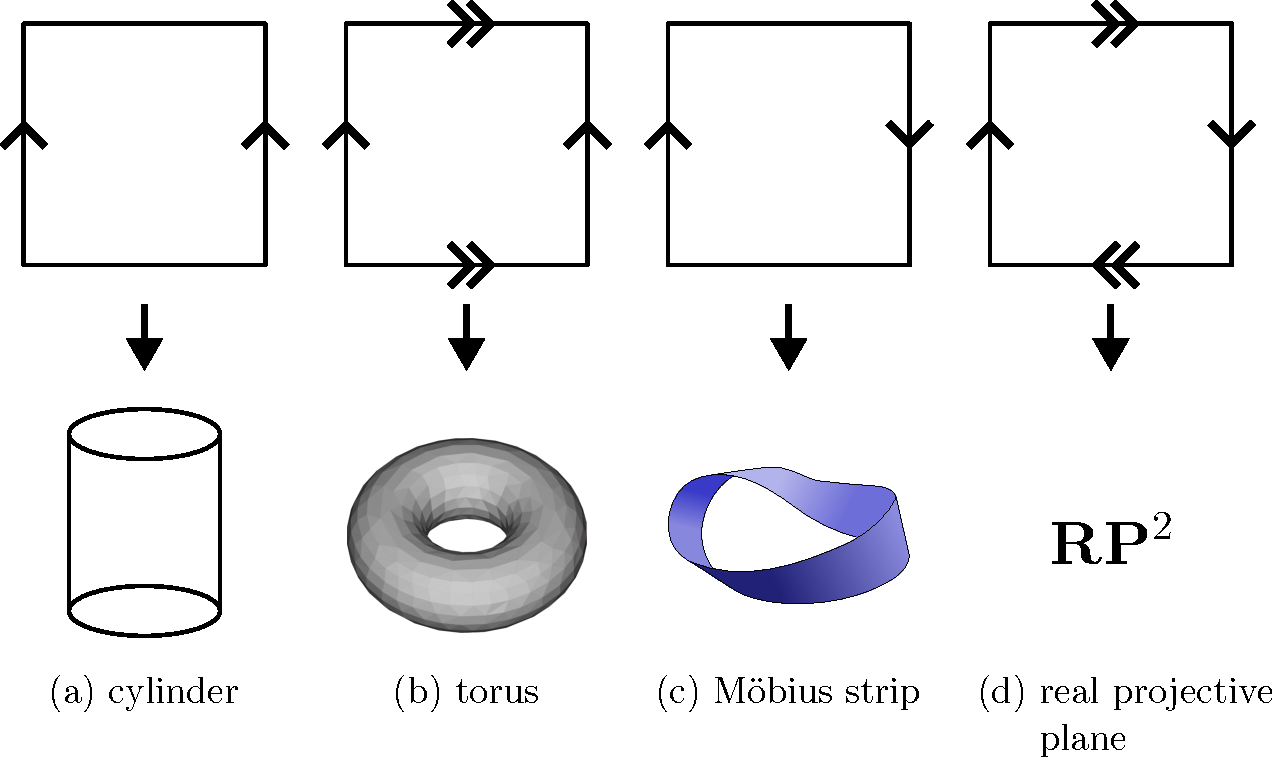
\includegraphics[width=0.8\linewidth]{topological-shapes.pdf}
	\caption{Visualization of topological shapes. 
	Arrows indicate which edges should be glued together and in which orientation (arrows should be aligned).}
	\label{fig:shapes}
\end{figure}

Here is a visualization I find helpful and it might aid your learning as well.
Imagine we have a rectangular piece of paper that we're trying to transform into a 3D shape.
There are many ways to do this, so to guide the construction, we will draw arrows along opposite edges and their orientation determines how we will join (e.g., glue) the two edges together to turn the 2D paper into a 3D object.
For example, if we only draw upward pointing arrows on the left and right edges of the paper, then joining the two edges will form a cylinder, as illustrated in \autoref{fig:shapes}a.
Closely study the other examples shown to convince yourself that the shapes can be formed as claimed---again, it might be helpful to get some paper and try it!

Left/right $\rightarrow$ cylinder.
Left/right, top/bottom $\rightarrow$ torus.
Left/right with twist $\rightarrow$ M{\"o}bius strip
Left/right, top/bottom, both with twist $\rightarrow$ $\mathbf{RP}^2$, real projective plane.
Hard to visualize!
Yes this is the topological space that defines how indistinguishable particles behave!

We can classify these spaces using something called the \textbf{fundamental group}.\footnote{While long, the \href{https://en.wikipedia.org/wiki/Fundamental_group}{Wikipedia page} on the fundamental group has many nice visuals.}
It classifies the types of curves/paths in a topological space by ``measuring the number of holes" (loosely speaking) in the geometric object.
For example, take the sphere in three dimensions, which we symbolize with $S^2$ (the `2' refers to a 2D surface).

\begin{figure}[!ht]
	\centering 
	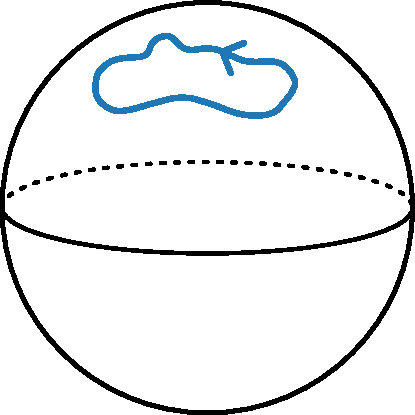
\includegraphics[width=0.4\linewidth]{sphere-closed-curve.pdf}
	\caption{Closed curve on sphere.}
	\label{fig:sphere1}
\end{figure}

The blue curve in \autoref{fig:sphere1} (and all closed curves on the sphere) can be contracted to a point on its surface (the null curve).
Therefore, we say that all closed curves are \emph{homotopic} to the null curve, as defined previously.
Using the notation of topology, where the fundamental group is denoted\footnote{`1' for the first homotopy group, $\pi$ likely for its discover, Henri Poincar{\'e}.} by $\pi_1$, we would say 

\begin{equation*}
	\pi_1(S^2) = 0
\end{equation*}

Similarly, if we look at a 2D plane in the Cartesian coordinate system (denoted $R^2$), all closed curves in the plane can also be contracted to a point, and thus there are no holes.
We would denote this in a similar way, 

\begin{equation*}
	\pi_1(R^2) = 0
\end{equation*}

While these examples might seem straightforward, the fundamental group isn't always so trivial.
Consider now the circle in 2D, symbolized by $S^1$, and shown in \autoref{fig:circle1}.

\begin{figure}[!ht]
	\centering 
	\subfloat[]{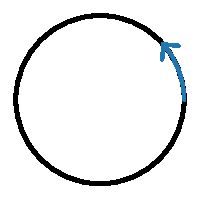
\includegraphics[width=0.31\linewidth]{circle-null-curve.pdf} \label{fig:circle1a}} \hfill
	\subfloat[]{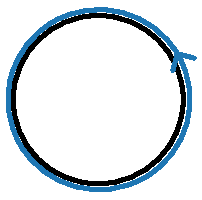
\includegraphics[width=0.31\linewidth]{circle-1-curve.pdf} \label{fig:circle1b}} \hfill
	\subfloat[]{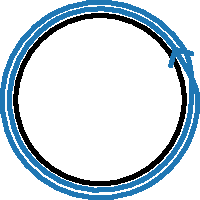
\includegraphics[width=0.31\linewidth]{circle-2-curve.pdf} \label{fig:circle1c}}
	\caption{Curves on a circle.
	(a) The null curve, which is contractable (homotopic) to a point.
	(b) A knotted curve with a winding number of 1.
	(c) A curve with two loops cannot be contracted to either of the previous two. 
	This path has a winding number of 2.}
	\label{fig:circle1}
\end{figure}

In panel~\ref{fig:circle1a}, we have drawn a small arc that is homotopic to a point when contracted. 
In panel~\ref{fig:circle1b}, we have a single loop around the circle.
This curve is knotted! 
It cannot be contracted to a point, and we quantify its properties using a \emph{winding number} of 1.
Similarly, in panel~\ref{fig:circle1b}, we have two loops around the circle.
This is yet another distinct case, as there's no way to contract this double loop into a single loop or the null curve. 
In fact, we can characterize it with a winding number of 2.

By now you probably see the pattern. 
The \href{https://en.wikipedia.org/wiki/Winding_number}{winding number} can be positive or negative depending on whether the loops are counterclockwise or clockwise around the circle, respectively.
Thus we can have a distinct loop/curve for every positive or negative integer.
We say that $\pi_1(S^2) = \mathbb{Z}$, which is the group of integers.
In this way, the fundamental group is powerful because it lets us classify different topological spaces using an algebraic quantity.

\begin{figure}[!ht]
	\centering 
	\subfloat[]{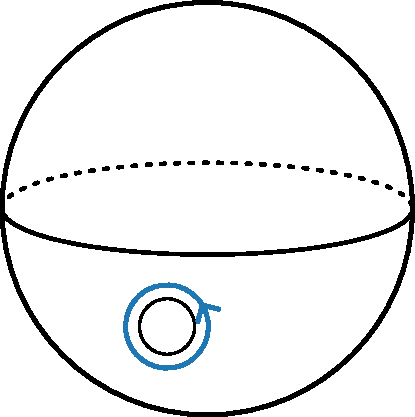
\includegraphics[width=0.35\linewidth]{sphere-1-hole.pdf} \label{fig:sphere2a}} \hspace{6ex}
	\subfloat[]{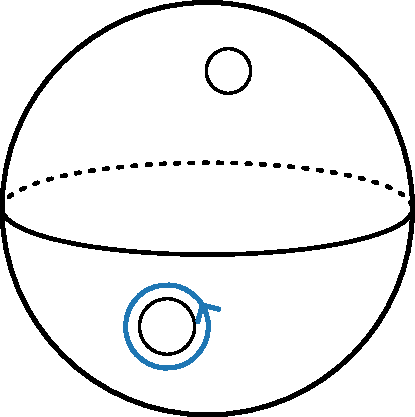
\includegraphics[width=0.35\linewidth]{sphere-2-hole.pdf} \label{fig:sphere2b}}
	\caption{(a) A punctured sphere with a single hole, where all loops on the surface are trivial.
	(b) A double-punctured sphere, where the same loop is no longer trivial.}
	\label{fig:sphere2}
\end{figure}

Let's do a few more examples. 
Consider the \emph{punctured} sphere, which is a sphere with a hole cut in it (Figure~\ref{fig:sphere2a}).
All loops, even those which enclose the hole (example shown in blue) are trivial.
Such a loop can be expanded outward and then collapsed on the \emph{other side} of the sphere!
Indeed, the punctured sphere is \emph{homeomorphic}\footnote{This is similar to homotopy equivalence, but \href{https://en.wikipedia.org/wiki/Homotopy\#Homotopy_equivalence_vs._homeomorphism}{slightly stronger}. Sorry for so many terms!} to a disc $D^2$.
There exists a continuous deformation which collapses a punctured sphere to a flat 2D disc.
Note here we use a different notation because a disc includes all the points inside the circle, whereas the circle $S^1$ is just the boundary.

Figure~\ref{fig:sphere2b} is another example, this time a double punctured sphere.
Now a loop around one hole gets caught on the other during the attempted collapse of the loop.
In fact, this space is homeomorphic to a punctured disc, which in turn is just the circle $S^1$!\footnote{Can you picture this? What if you start with an annulus and then make it thinner?} 
Thus the fundamental group of the twice-punctured sphere is also $\mathbb{Z}$.


%%%%%%%%%%%%%%%%%%%%%%%%%%%%%%%%%%%%%%%%%%%%%%%%%%%%%%%%%%%%%%%%%%%%%%%%%%%%%%%%

\section{Back to fermions}

That was exciting! (hopefully)
Time to bring back the science.
In 3D, let's consider the 2-particle configuration space for fermions.
We can define this by the relative coordinate $\vec{r} = \vec{r}_1 - \vec{r}_2$, where $\vec{r}_1$ and $\vec{r}_2$ are vectors pointing at the two particles (i.e., their positions).
By the Pauli exclusion principle, we know that $\vec{r} \neq 0$.

Furthermore, let's consider for simplicity (and without loss of generality\footnote{Theorists use this phrase when constructing an argument that uses a specific example or assumptions, but the result is generally valid, as other possible assumptions are equivalent by symmetry.}) the case where $\abs{\vec{r}}$ is fixed (topology allows for continuous deformations to enable this).
Then we would have a sphere!

\begin{figure}[!ht]
	\centering 
	\subfloat[]{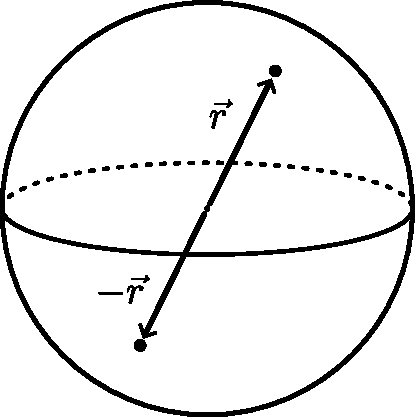
\includegraphics[width=0.4\linewidth]{sphere-antipodes.pdf}} \hspace{5ex} 
	\subfloat[]{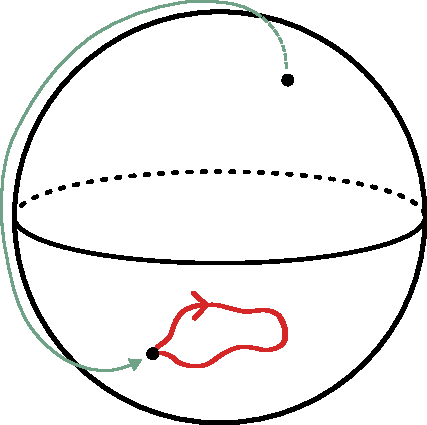
\includegraphics[width=0.42\linewidth]{sphere-antipodes-null-curve.pdf}}
	\caption{Antipodes on a sphere.}
	\label{fig:sphere3}
\end{figure}

Now let's look at the setup in \autoref{fig:sphere3}a, where $\vec{r}$ and $-\vec{r}$ are \textbf{antipodal points} on the sphere.
If we let $\vec{r} = \vec{r}_1 - \vec{r}_2$, which again we can always get by manipulating the particles' positions, then exchanging the two particles would produce $-\vec{r}$.

If the particles are indistinguishable, then the topological space we have for this 2-particle system is a sphere with antipodal points identified.\footnote{Which, as alluded to before, is the definition of the space RP$^2$, as explained nicely \href{https://www.popmath.org.uk/sculpmath/pagesm/plane.html}{here}.}

Now we might ask: What is this space?
Let's revisit our original activity by considering paths in this space that represent the motion of the two particles, such as the red path in \autoref{fig:sphere3}b.
We've already seen how such a path is homotopic to the null loop as it can be collapsed to a point.

\begin{figure}[!ht]
	\centering 
	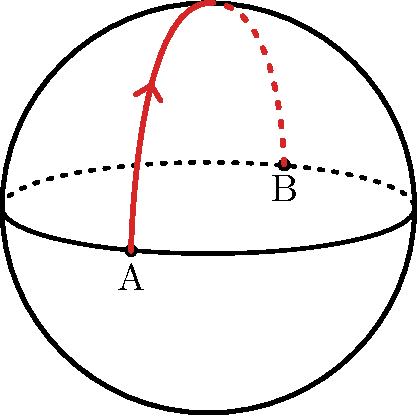
\includegraphics[width=0.4\linewidth]{sphere-single-exchange.pdf}
	\caption{Single exchange on a sphere.}
	\label{fig:sphere-exchange}
\end{figure}

Now consider the path in \autoref{fig:sphere-exchange}, which sends $\vec{r} \rightarrow -\vec{r}$ and corresponds to an exchange.
It is a closed loop in this space!
We travel from $A$ to $B$ along the curve, and then because $B$ is identical to $A$, we go through a portal back to $A$! 
This curve cannot be contracted to a point while keeping the ends fixed.
This is the path associated with an exchange operation, or rotation by $2\pi$.

\begin{figure}[!ht]
	\centering 
	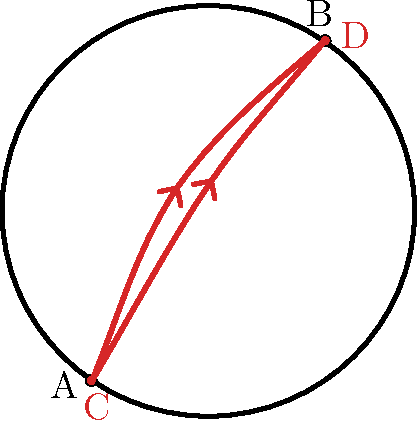
\includegraphics[width=0.4\linewidth]{sphere-double-exchange-top.pdf}
	\caption{Double exchange on a sphere. (top view)}
	\label{fig:sphere-double}
\end{figure}

Next, let's consider double exchange, which we draw in \autoref{fig:sphere-double}. 
Again we begin by traveling from $A$ to $B$, which sends us back to $A$.
This time, we label this new (equivalent) point $C$.
Now we travel from $C$ to $D$, where the latter is equivalent to the original point $B$. 
This is the loop associated with double exchange, or a rotation by $4\pi$.

\begin{figure}[!ht]
	\centering 
	\subfloat[]{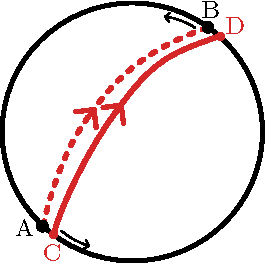
\includegraphics[width=0.23\linewidth]{sphere-double-exchange-1.pdf} \label{fig:sphere-double2a}} \hfill
	\subfloat[]{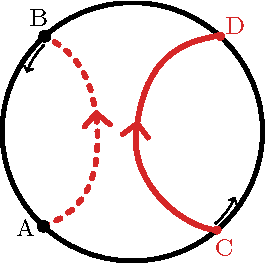
\includegraphics[width=0.23\linewidth]{sphere-double-exchange-2.pdf} \label{fig:sphere-double2b}} \hfill
	\subfloat[]{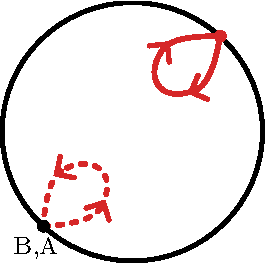
\includegraphics[width=0.23\linewidth]{sphere-double-exchange-3.pdf} \label{fig:sphere-double2c}} \hfill
	\subfloat[]{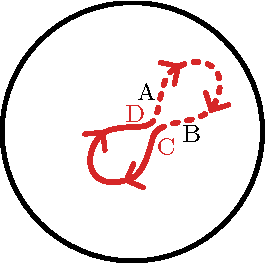
\includegraphics[width=0.23\linewidth]{sphere-double-exchange-4.pdf} \label{fig:sphere-double2d}}
	\caption{Double exchange process on a sphere.}
	\label{fig:sphere-double2}
\end{figure}

How might we perform a continuous deformation of this closed double loop from $A$ to $D$?
\autoref{fig:sphere-double2} attempts to illustrate this process.
We start with the configuration in \ref{fig:sphere-double2a} and we move points $B$ and $C$ along the equator in opposite directions, away from $D$ and $A$, respectively (\ref{fig:sphere-double2b}). 
Note that during this process, $B$ and $C$ remain antipodes and $A$ and $D$ are fixed in place, so we have not broken the topology of the system; such a continuous deformation was not possible previously when we only had $A$ and $B$ as endpoints (\ref{fig:sphere-exchange}).
We proceed with this process until $B$ coincides with $A$ and $C$ coincides with $D$, effectively closing two smaller loops on the surface of the sphere (\ref{fig:sphere-double2c}). 
Finally, in a feat of quantum magic, we pull the loop at $A$,$B$ through the antipodal portal to the other side, resulting in panel \ref{fig:sphere-double2d}.
Now we have a trivial, contractable loop $ABCD$ that is homotopic to null.
Thus there are only 2 classes of topologically inequivalent closed paths in 3D, corresponding to fermions and bosons.
In topology notation, we write $\pi_1(\mathrm{RP}^2) = \mathbb{Z}_2$, where $\mathbb{Z}_2$ denotes the cyclic group of order 2.\footnote{Sometimes $\mathbb{Z}_2$ is also written as $\mathbb{Z}/2\mathbb{Z}$.}
This means that the group can be generated using just two elements of its members, $I$ and $X$, with $X^2 = I$.
We have now arrived back to the beginning of the chapter, with a much more complex, topological view of the statement $e^{2i \alpha} = 1$!

\begin{figure}[!ht]
	\centering 
	\subfloat[]{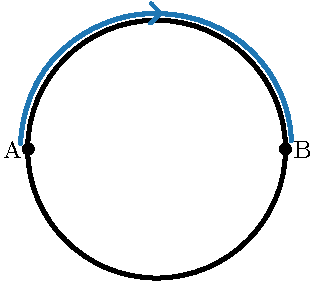
\includegraphics[width=0.4\linewidth]{circle-single-exchange.pdf} \label{fig:circle-exchange-a}} \hspace{6ex}
	\subfloat[]{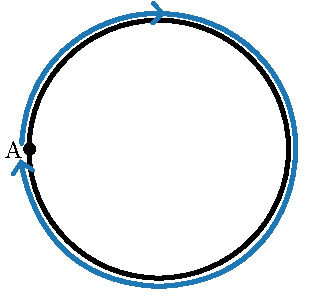
\includegraphics[width=0.4\linewidth]{circle-double-exchange.pdf} \label{fig:circle-exchange-b}}
	\caption{Antipodes on a circle.}
	\label{fig:circle-exchange}
\end{figure}

Before we wrap up, let's go down a dimension into 2D.
This configuration space is a circle with opposite points identified (RP$^1$).
As illustrated in Figure~\ref{fig:circle-exchange-a}, the path $A \rightarrow B$ is a closed loop (as $A$ and $B$ are antipodes) and corresponds to the exchange operation in 2D.
Performing double exchange takes us all the way around the circle, as shown in panel~\ref{fig:circle-exchange-b}.
Note this is still topologically distinct.

Generalizing, under $n$ exchanges, we just wrap $n$ times around.
The winding number is $n$ and just like above, we can say $\pi_1 (\mathrm{RP}^1) = \mathbb{Z}$.
Thus, if we pick up a phase factor $e^{i\alpha}$ on each exchange, there is no requirement that $e^{2i \alpha} = 1$.
This is the anyon case!


\subsection{Notes on spin statistics}

In the previous discussion, the essence of the argument comes down to the following picture (Figure~\ref{fig:loop-twist-a}).
In 3D, it would seem that the left loop is equivalent to the right.
If we just pull on it, it straightens out, as one might expect with a string.

\begin{figure}[!ht]
	\centering 
	\subfloat[]{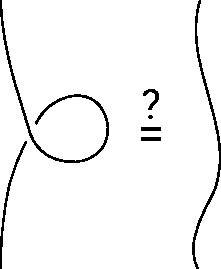
\includegraphics[height=2.5in]{twist-thin.pdf} \label{fig:loop-twist-a}} \hspace{8ex} 
	\subfloat[]{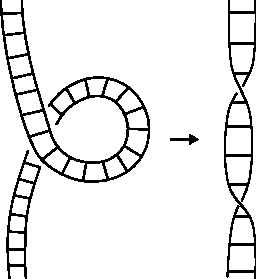
\includegraphics[height=2.5in]{twist-thick.pdf} \label{fig:loop-twist-b}}
	\caption{Twisted loops thin and thick.}
	\label{fig:loop-twist}
\end{figure}

In fact, however, these two objects are \emph{not} topologically equivalent.
Imagine a string with finite diameter (Figure~\ref{fig:loop-twist-b}).
If we try to pull this string straight, the loop is gone, yes, but we would also get a double twist along the length of the string.\footnote{A similar thing happens if we try to straighten a garden hose.}
This is the fact that underlies how we get nontrivial phases under exchange.


Our motivation for studying the fundamental group is to prove that the fundamental group of $SO(3)$, the group of rotations, is a cyclic group of order two. 
In physics applications this result is interesting to us because it is associated to spin and spinor representations in quantum mechanics. 
It explains why a rotation body can have a spin of half a quantum and no other fraction.



%%%%%%%%%%%%%%%%%%%%%%%%%%%%%%%%%%%%%%%%%%%%%%%%%%%%%%%%%%%%%%%%%%%%%%%%%%%%%%%%

\section{Application: Topological insulators}

TODO. 
If you've stuck with us all the way to this point, major kudos.

https://www.youtube.com/watch?v=6ebiyOtn7NA knots video applications

Joel Moore, Nature: https://www.nature.com/articles/nature08916
Qi and Zhang, Rev Modern Phys: https://link.aps.org/doi/10.1103/RevModPhys.83.1057
Hasan and Kane, Rev Modern Phys: https://link.aps.org/doi/10.1103/RevModPhys.82.3045
Ando, intro, Japan: https://journals.jps.jp/doi/abs/10.7566/JPSJ.82.102001
Choi, true intro, IEEE Spectrum: https://spectrum.ieee.org/a-beginners-guide-to-topological-materials

Electronic topological insulators: bismuthene.

Photonic topological insulators: Layers of GaAs and AlGaAs.

Topological superconductors: superconducting metal + semiconductor, producing Majorana fermions.

Topological semimetals: TaAs, CoSi, Dirac semimetals, Weyl semimetals, etc.


%%%%%%%%%%%%%%%%%%%%%%%%%%%%%%%%%%%%%%%%%%%%%%%%%%%%%%%%%%%%%%%%%%%%%%%%%%%%%%%%

\section{Summary}
To recap, in this chapter we analyzed...

%} % for doublespacing
\end{document}